\documentclass[letterpaper, 10pt, DIV=13]{scrartcl}
\usepackage[T1]{fontenc}
\usepackage[english]{babel}
\usepackage{amsmath, amsfonts, amsthm, xfrac}
\usepackage{listings}
\usepackage{color}
\usepackage{longtable}

\numberwithin{equation}{section}
\numberwithin{figure}{section}
\numberwithin{table}{section}

\usepackage{sectsty}
\allsectionsfont{\normalfont\scshape} % Make all section titles in default font and small caps.

\usepackage{fancyhdr} % Custom headers and footers
\pagestyle{fancyplain} % Makes all pages in the document conform to the custom headers and footers

\fancyhead{} % No page header - if you want one, create it in the same way as the footers below
\fancyfoot[L]{} % Empty left footer
\fancyfoot[C]{} % Empty center footer
\fancyfoot[R]{\thepage} % Page numbering for right footer

\renewcommand{\headrulewidth}{0pt} % Remove header underlines
\renewcommand{\footrulewidth}{0pt} % Remove footer underlines
\setlength{\headheight}{13.6pt} % Customize the height of the header

\setlength\parindent{0pt}
\pagenumbering{gobble}

\title {
	\normalfont
	\huge{Lab 2} \\
	\vspace{10pt}
	\large{CMPT 432 - Spring 2023 | Dr. Labouseur}
}

\author{\normalfont Josh Seligman | joshua.seligman1@marist.edu}

\pagenumbering{arabic}

\definecolor{mygreen}{rgb}{0,0.6,0}
\definecolor{mygray}{rgb}{0.5,0.5,0.5}
\definecolor{mymauve}{rgb}{0.58,0,0.82}
\lstset{
  backgroundcolor=\color{white},   % choose the background color
  basicstyle=\footnotesize,        % size of fonts used for the code
  breaklines=true,                 % automatic line breaking only at whitespace
  captionpos=b,                    % sets the caption-position to bottom
  commentstyle=\color{mygreen},    % comment style
  escapeinside={\%*}{*},          % if you want to add LaTeX within your code
  keywordstyle=\color{blue},       % keyword style
  stringstyle=\color{mymauve},     % string literal style
}

\begin{document}
\maketitle

\section{Crafting a Compiler}
\subsection{Exercise 3.3}
Write regular expressions that define the strings recognized by the FAs: \\
\begin{figure}[ht]
    \centering
    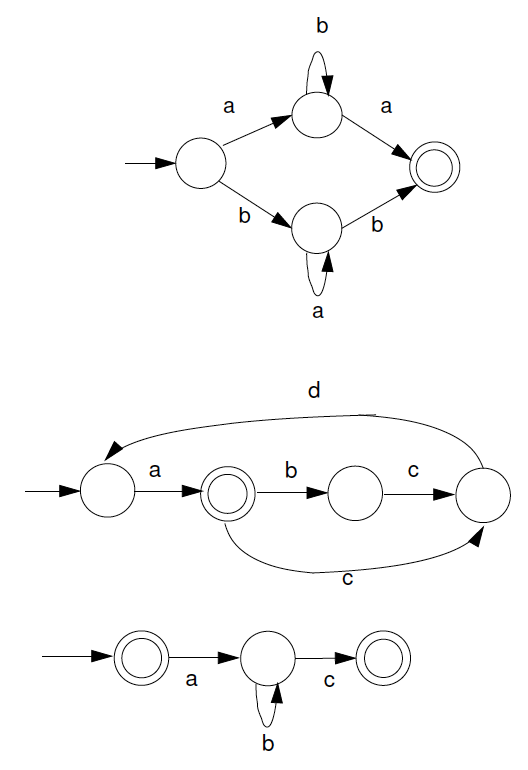
\includegraphics[height=10cm]{cac3_3}
\end{figure}
\begin{enumerate}
    \item $(ab^*a)|(ba^*b)$
    \item $a(b?cda)^*$
    \item $(ab^*c)?$
\end{enumerate}

\subsection{Exercise 3.4}
Write DFAs that recognize the tokens defined by the following regular expressions:
\begin{figure}[ht]
    \centering
    \includegraphics[width=12cm]{cac3_4}
\end{figure}

\section{Dragon}
\subsection{Exercise 3.3.4}
Most languages are case sensitive, so keywords can be written only one way, and the regular expressions describing their lexeme is very simple. However, some languages, like SQL, are case insensitive, so a keyword can be written either in lowercase or in uppercase, or in any mixture of cases. Thus, the SQL keyword SELECT can also be written select, Select, or sElEcT, for instance. Show how to write a regular expression for a keyword in a case insensitive language. Illustrate the idea by writing the expression for "select" in SQL. \\\\

Brute force method: (S|s)(E|e)(L|l)(E|e)(C|c)(T|t) \\
Easier approach: Use the i flag at the end for case insensitive match: /select/i

\end{document}